\documentclass[journal,12pt,twocolumn]{IEEEtran}
\usepackage[utf8]{inputenc}
\usepackage{amsmath}
\usepackage{amssymb}
\usepackage{graphicx}
\usepackage{tcolorbox}
\providecommand{\brak}[1]{\ensuremath{\left(#1\right)}}

\title{Assignment 2}
\author{ADEPU VASISHT}
\date{March 2021}

\begin{document}

\maketitle

\section*{GATE EC Problem 30}
If E denotes the expectation, the variance of a random variable X is given by ?

\begin{description}
\item[$\brak{A}$]$E[X^2]-E^2[X]$ 
\item[$\brak{B}$]$E[X^2]$
\item[$\brak{C}$]$E[X^2]+E^2[X]$ 
\item[$\brak{D}$]$E^2[X]$
\end{description}

\section*{Solution}
The expectation of a random variable X is given by
\begin{equation}
E[X]=\sum_{all \ x}x\Pr\brak{x}=\mu
\end{equation} 
The variance of the random variable X is given by
\begin{equation}
Var\brak{X}=\sum_{all \ x}\brak{x-\mu}^2\Pr\brak{x}
\end{equation} 
We know that sum of all the probabilities is 1 i.e
\begin{equation}
\sum_{all \ x}\Pr\brak{x} = 1
\end{equation}

We expand the variance equation $\brak{2}$ from above
\begin{align}
\nonumber Var\brak{X}&=\sum_{all \ x}\brak{x-\mu}^2\Pr\brak{x}\\\nonumber\\\nonumber
&= \sum_{all \ x}\brak{x^2-2x\mu+\mu^2}\Pr\brak{x}\\\nonumber\\\nonumber
&= \sum_{all \ x}x^2\Pr\brak{x}-2\mu\sum_{all \ x}\Pr\brak{x}\\\nonumber
&\qquad  +\mu^2\sum_{all \ x}\Pr\brak{x}\\\nonumber\\\nonumber
&= E[X^2]-2\mu\cdot\mu+ \mu^2\brak{1} \brak{\because \brak{1} and \brak{3}}\\\nonumber\\\nonumber
&= E[X^2]-E^2[X]
\end{align}

Hence option A is the correct answer







\section*{Graph using Python}
We consider a binomial distribution with random variable X and assign randomly the values it can take and probability is also random. We calculate two variances one using the formula $Var\brak{X}=E[X^2]-E^2[X]$ and other using the inbuilt function in scipy.stats. We plot the graph between two and compare them with the line $x=y$. With the green points representing the variance points.

\begin{figure}[ht]
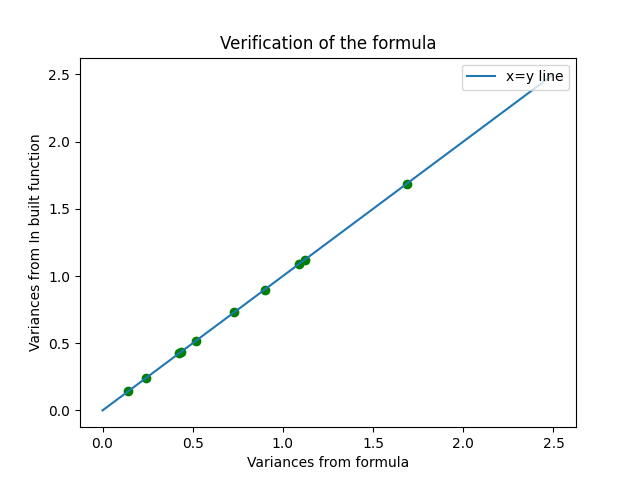
\includegraphics[scale = 0.7]{ogimage}]
\end{figure}
As we can see from the above graph all the points lie on the line $x=y$ so the formula is correct \\\\




\end{document}
